\documentclass[omni.tex]{subfiles}

\begin{document}

\begin{figure}
{\begin{center}
    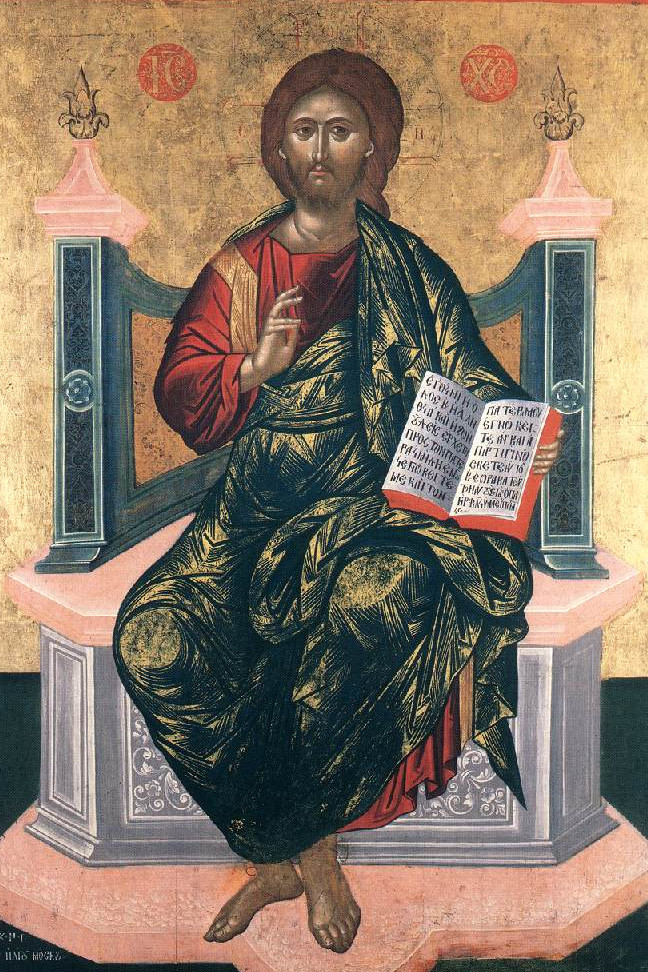
\includegraphics[width=2in]{pantocrator_moskos}
\end{center}}
\end{figure}

\poemtitle{Laud\'ate D\'ominum \\ (Psalmus 116)}
\settowidth{\versewidth}{Et ne nos ind\'ucas in tentati\'onem}

\begin{verse}[\versewidth]
\lettrine[lhang=1.0,nindent=0em]{L}{aud\'ate D\'ominum}, \\> 
omnes gentes; \\>
laud\'ate eum, omnes p\'opuli.
\end{verse}

\begin{verse}[\versewidth]
Qu\'oniam confirm\'ata est \\
super nos miseric\'ordia eius, \\
et v\'eritas D\'omini manet \\
in \ae t\'ernum. \\
Amen. \\[6\baselineskip]
\end{verse}
\attrib{VII}

\pagebreak
\end{document}
